% -*- mode: noweb; noweb-default-code-mode: R-mode; -*-








\graphicspath{ {datasets/} }

\begin{Schunk}
\begin{Sinput}
>                                         # load helper functions
>                                         # code will appear in appendix
> source("~/thesis/code/peel.R")
> setwd( "~/thesis/datasets")
> ##setwd( "/gpfs/pads/projects/see/nbest/thesis/data")
> ##quartz.options( type="png")
> 
> overwriteRasters <- FALSE
> overwriteFigures <- FALSE
> 
\end{Sinput}
\end{Schunk}

\chapter{Data}
\label{cha:data}

This chapter presents some summary descriptions of the various data
sets that are relevant to this analysis and further discussion on how
they were manipulated.

The general approach with the classified land cover data sets (MLCT,
NLCD, CDL) is to reclassify their categories and aggregate the new
classification to the 5-arcmin grid.  The purpose of the
reclassification is to reduce the number of classes and have a uniform
set of classes across data sets.  The challenge in this is that
classification defintions are sometimes subtly different which makes
direct comparison across data sets difficult.  In this process we
convert classified maps whose pixels have discrete values to a stack
of maps, one map per class, whose pixels have real number values on
the interval $[0,1]$ and are constrained to sum to unity for each
pixel through the stack.  In the general case of the MLCT data product
the process converts two discrete, thematic variables and one
continuous variable, those being a primary covery type, a secondary
cover type, and classification confidence level respectively, into a
set of continuous variables representing fractional areas for the
cover types in the siplified classification system.  In other cases
the process is simplified by considering only a primary thematic layer
and performing the aggregation without a secondary cover type or
confidence level by which to relate them.

\missingfigure{Generate a summary table of data sets (raster/tabular, resolution, citation)}

\section{MODIS Land Cover Type (MLCT)}
\label{sec:mlct}

In preparation for this analysis we prepared the 2001 MLCT data by patching
together the tiles as delivered in the equal-area sinusoidal
projection, reprojecting that mosaic to geographic coordinates, and
extracting a subset for the conterminous United States (cUSA).  The
subset is defined as the set of 5-arcmin grid cells that intersect
with the cUSA polygon in the Global Administrative Areas (GADM) vector
data set, which includes the water bodies on the American side of the
international border across the Great Lakes, but does not extend to
oceanic waters beyond the coastal grid cells that intersect with the
land mass.  

The expectation is that the analytical approach developed here will be
applied globally in the future.

To illustrate the process of converting the MLCT data from its
original representation we are including maps of an area of
southeastern Michigan to show greater detail through each step of the
process.  We chose this region for its diversity of land covers and
uses, diveristy of agricultural commodities across its significant
cropland area, and its familiarity to our principal author, being his
brthplace.  In this section we will demonstrate the process of
converting the MLCT data from its native form, consisting of primary
cover type, classification confidence for the primary cover, and
secondary (alternate) cover type at 15-arcsec resolution, to a stack
of cover fractions at 5-arcmin resolution using the simplified
cover/use classification specified by the PEEL model. 

\begin{Schunk}
\begin{Sinput}
> ## this works but it's slow
> ##
> ## thumb <- crop( raster("2001_lct1.tif"), 
> ##                extent(-83.5, -(82+25/60), 42+55/60, 44+5/60))
> ##
> 
> ## these are subsets exported from GRASS
> 
> texWd <- setwd("../data")
> dataWd <- getwd()
> thumb <- mlctList( "thumb_2001_lct1.tif", 
+                    "thumb_2001_lct1_sec.tif", 
+                    "thumb_2001_lct1_pct.tif")
> igbpLegend <- thumb$pri@legend@colortable
> igbpLegend <- igbpLegend[ igbpLegend != "#000000"]
> 
> ## just in case, save these for later
> ##  paste( deparse( igbpLegend), collapse="")
> ## igbpLegend <- c("#2041B3", "#006A0F", "#007C25", "#00A25B", "#00A125", "#069228", "#9E9668", "#C1C48F", "#85AA5B", "#B1B741", "#A4D07E", "#73ABAE", "#CCD253", "#D90000", "#9DE36E", "#B6B5C2", "#949494")"
> 
\end{Sinput}
\end{Schunk}
\subsection{Reclassification}
\label{sec:mlct-reclass}

The following table shows the mapping of the IGBP classes used in the
original MLCT data to the simplified classification designed for the
PEEL model.

\missingfigure{MLCT reclassification table}


\begin{Schunk}
\begin{Sinput}
> thumb <- mlctReclass( thumb, mlctReclassMatrix, overwrite= overwriteRasters)
> if( overwriteFigures) {
+   thumbPlots <- list( pri= peelMap( thumb$pri, 0.4),
+                      sec= peelMap( thumb$sec, 0.4))
+ 
+   thumbPlots$pct <- ggplotRaster( thumb$pct, 0.4) + 
+     scale_fill_gradientn( "% confidence", 
+                          colours= rev( brewer.pal( 7, "YlGn")), 
+                          limits= c( 100, 0),
+                          breaks= seq( 100, 0, by= -20))
+ }
> 
\end{Sinput}
\end{Schunk}

\subsubsection{Detail Area}
\label{sec:reclass-detail-area}


The following figures show the result of reclassifying the MLCT data
for our detailed study area along with the confidence level given for
the primay classification.

\begin{figure} 
\begin{center}
  
\begin{Schunk}
\begin{Sinput}
> setwd( texWd)
> if( overwriteFigures) {
+   png( file="fig_thumb_pri_reclass.png")
+   print( thumbPlots$pri)
+   dev.off()
+ }
> 
\end{Sinput}
\end{Schunk}

\includegraphics{fig_thumb_pri_reclass}
\end{center} 
\caption{MLCT primary cover reclassified detail} 
\label{fig:thumb_pri_reclass} 
\end{figure} 


\begin{figure} 
\begin{center}
  
\begin{Schunk}
\begin{Sinput}
> setwd( texWd)
> if( overwriteFigures) {
+   png( file="fig_thumb_sec_reclass.png")
+   print( thumbPlots$sec)
+   dev.off()
+ }
> 
\end{Sinput}
\end{Schunk}

\includegraphics{fig_thumb_sec_reclass}
\end{center} 
\caption{MLCT secondary cover reclassified detail} 
\label{fig:thumb_sec_reclass} 
\end{figure} 


\begin{figure} 
\begin{center}
  
\begin{Schunk}
\begin{Sinput}
> setwd( texWd)
> if( overwriteFigures) {
+   png( file="fig_thumb_pct.png")
+   print( thumbPlots$pct)
+   dev.off()
+ }
> 
\end{Sinput}
\end{Schunk}

\includegraphics{fig_thumb_pct}
\end{center} 
\caption{MLCT primary cover classification confidence} 
\label{fig:thumb_pct} 
\end{figure} 

It is easier to see the relative proportions of the primary and
secondary cover types if we map them separately.  These maps show that
this region is dominated by the cropland and cropland/natural
vegetation mosaic cover types with scattered forests and towns.
Shrub, wetland, barren, and open covers are found sparsely along the
shore of Lake Huron.  The urban center of Port Huron is visible in the
southeast corner.

\begin{figure} 
\begin{center}
  
\begin{Schunk}
\begin{Sinput}
> setwd( texWd)
> if( overwriteFigures) {
+   png( file="fig_thumb_pri_facet.png")
+   print( thumbPlots$pri + 
+         facet_wrap(~ values) + 
+         opts( legend.position= "none"))
+   dev.off()
+ }
> 
\end{Sinput}
\end{Schunk}

\includegraphics{fig_thumb_pri_facet}
\end{center} 
\caption{MLCT primary covers shown separately, detail} 
\label{fig:thumb_pri_reclass} 
\end{figure} 


\begin{figure} 
\begin{center}
  
\begin{Schunk}
\begin{Sinput}
> setwd( texWd)
> if( overwriteFigures) {
+   png( file="fig_thumb_sec_facet.png")
+   print( thumbPlots$sec + 
+         facet_wrap(~ values) +
+         opts( legend.position= "none"))
+   dev.off()
+ }
> 
\end{Sinput}
\end{Schunk}

\includegraphics{fig_thumb_sec_facet}
\end{center} 
\caption{MLCT secondary covers shown separately, detail} 
\label{fig:thumb_pri_reclass} 
\end{figure} 

\subsubsection{Analysis Area}
\label{sec:reclass-analysis-area}

We repeat this operation for the entire data set.


\begin{Schunk}
\begin{Sinput}
> ## repeat for cUSA
> setwd( dataWd)
> mlct <- mlctList( "2001_lct1.tif", 
+                   "2001_lct1_sec.tif", 
+                   "2001_lct1_pct.tif")
> mlct  <- mlctReclass( mlct, mlctReclassMatrix, overwrite= overwriteRasters, datatype="INT1U", progress="text")
> if( overwriteFigures) {
+   mlctPlots <- list( pri= peelMap( mlct$pri, 0.01),
+                     sec= peelMap( mlct$sec, 0.01))
+   mlctPlots$pct <- ggplotRaster( mlct$pct, 0.01) + 
+     scale_fill_gradientn( "% confidence", colours=rev( brewer.pal( 7, "YlGn")), 
+                          limits= c( 100, 0),
+                          breaks= seq( 100, 0, by= -20))
+ }
> 
> 
\end{Sinput}
\end{Schunk}

\begin{figure} 
\begin{center}

\begin{Schunk}
\begin{Sinput}
> setwd( texWd)
> if( overwriteFigures) {
+   png( file="fig_mlct_pri_reclass.png")
+   print( mlctPlots$pri + coord_equal())
+   dev.off()
+   system( "convert -trim fig_mlct_pri_reclass.png fig_mlct_pri_reclass_trim.png")
+ }
> 
\end{Sinput}
\end{Schunk}

\includegraphics{fig_mlct_pri_reclass_trim}
\end{center} 
\caption{MLCT primary cover reclassified} 
\label{fig:mlct_pri_reclass} 
\end{figure} 


\begin{figure} 
\begin{center}
  
\begin{Schunk}
\begin{Sinput}
> setwd( texWd)
> if( overwriteFigures) {
+   png( file="fig_mlct_sec_reclass.png")
+   print( mlctPlots$sec + coord_equal())
+   dev.off()
+   system( "convert -trim fig_mlct_sec_reclass.png fig_mlct_sec_reclass_trim.png")
+ 
+ }
> 
\end{Sinput}
\end{Schunk}

\includegraphics{fig_mlct_sec_reclass_trim}
\end{center} 
\caption{MLCT secondary cover reclassified} 
\label{fig:mlct_sec_reclass} 
\end{figure} 


\begin{figure} 
\begin{center}
  
\begin{Schunk}
\begin{Sinput}
> setwd( texWd)
> if( overwriteFigures) {
+   png( file="fig_mlct_pct.png")
+   print( mlctPlots$pct + coord_equal())
+   dev.off()
+   system( "convert -trim fig_mlct_pct.png fig_mlct_pct_trim.png")
+ }
> 
\end{Sinput}
\end{Schunk}

\includegraphics{fig_mlct_pct_trim}
\end{center} 
\caption{MLCT primary cover classification confidence} 
\label{fig:mlct_pct} 
\end{figure} 

\todo{Fix artifacts in confidence figure}

\todo{Describe characteristics of MLCT reclass maps and confidence at
  cUSA extents}

\begin{figure} 
\begin{center}
  
\begin{Schunk}
\begin{Sinput}
> setwd( texWd)
> if( overwriteFigures) {
+   png( file="fig_mlct_pri_facet.png")
+   print( mlctPlots$pri + 
+         facet_wrap(~ values) + 
+         coord_equal() +
+         opts( legend.position= "none"))
+   dev.off()
+ }
> 
\end{Sinput}
\end{Schunk}

\includegraphics{fig_mlct_pri_facet}
\end{center} 
\caption{MLCT primary covers shown separately} 
\label{fig:mlct_pri_reclass} 
\end{figure} 


\begin{figure} 
\begin{center}
  
\begin{Schunk}
\begin{Sinput}
> setwd( texWd)
> if( overwriteFigures) {
+   png( file="fig_mlct_sec_facet.png")
+                                         # had to remove some NAs from the data
+   mlctPlots$sec$data <- mlctPlots$sec$data[ !is.na(mlctPlots$sec$data$values),]
+   print( mlctPlots$sec + 
+         facet_wrap(~ values) + 
+         coord_equal() +
+         opts( legend.position= "none"))
+   dev.off()
+ }
> 
\end{Sinput}
\end{Schunk}

\includegraphics{fig_mlct_sec_facet}
\end{center} 
\caption{MLCT secondary covers shown separately} 
\label{fig:mlct_pri_reclass} 
\end{figure} 


\subsection{Aggregation}
\label{sec:mlct-aggr}

This product has a nominal resolution of 500m and uses the 17 IGBP
land cover classes. The dataset consists of a primary classification,
along with a measure of confidence up to 100\%, and a secondary
classification.  The secondary cover type is given as the most likely
alternative to the primary type \citep{Friedl2010}, but for purposes
of our analysis we are taking a more probabilistic view and
incorporating all available information from the base data.  Because
we are aggregating the data up to 5-arcmin resolution there is no
expectation that the sub-pixel fractions at full resolution are
spaitally specific, but in the aggregate the characterization will be
nuanced by this additional information.  The primary class covers at
least roughly 50-60\% of a given pixel $x$, and this percent is almost
certainly a monotonically increasing function of the confidence
measure $c$.  \todo{cite email from Friedl}.  For the purposes of this
analysis we assume that this dependence is linear. Thus, for the
primary and secondary cover types in a pixel:

$$
A_p(x) = A_{min} + (1 - A_{min}) c(x)
$$
$$
A_s(x) = 1 - A_p(x)
$$

where $0.50 \le A_{min} \le 0.60$ is primarily chosen based on an
interpretation of $c$.  Given that there are only a handful of
examples of $c < 0.20$ (see figure XX for an example) \todo{crossref
  histograms showing confidence distribution}, setting $A_{min} =
0.50$ is both rational and prudent.  Certainly for a classification to
be considered the primary it must represent a bare majority of the
area covered by that pixel, and the distributions of confidences
indicate that the vast majority of pixels contain greater than 60\% of
their area in the primary under the rubric described above. The
equations are simplified as follows by assuming this value for
$A_{min}$.

$$
A_p(x) = \dfrac{1 + c}{2}
$$
$$
A_s(x) = 1 - A_p(x) = \dfrac{1-c}{2}
$$

Applying these formulae results in a map for each cover type where the
pixel values are the sub-pixel areas on the interval $[0,1]$.  The map
of the fraction of the primary cover type is visually equivalent to
that of the classification confidence level because the former is
simply a linear scaling and offset of the latter.  

By way of comparison we also consider the trivial case of settimg
$A_{min} = 1$ which indicates that the secondary cover is ignored
altogether and the primary cover is taken to represent 100\% of the
pixel area.

Computationally the process of converting the reclassified maps to
sub-pixel fractions at the desired 5-arcmin resolution is a three-step
process.  First we calculate the fraction of the primary cover type as
a function of the classification confidence as described above.  Next,
a sub-pixel fraction for each cover type is calculated at full
resolution, recognizing that the primary and secondary classes may be
identical after the reclassification, such as cases where the original
data indicated two different type of forests.  Aggregating to a
coarser resolution is a simple matter of calculating the mean of these
values over the intersecting pixels at the original resoution.
Because the desired 5-arcmin resolution is a multiple of the original
15-arcsec resolution the pixels are perfectly nested, which is
convenient for properly computing this mean.

\subsubsection{Detail Area}
\label{sec:agg-detail-area}

\begin{Schunk}
\begin{Sinput}
> setwd( dataWd)
> ## calculate cover fractions and aggregate for detail area
> 
> thumb  <- primaryFraction( thumb, Amin=0.5, overwrite= overwriteRasters, progress= "text")
> thumb1 <- primaryFraction( thumb, Amin=1.0, overwrite= overwriteRasters, progress= "text")
> thumb  <- coverFractions( thumb, overwrite= overwriteRasters, progress= "text")
> thumb1 <- coverFractions( thumb1, overwrite= overwriteRasters, progress= "text")
> thumb  <- aggregateFractions( thumb, overwrite= overwriteRasters, progress= "text")
> thumb1 <- aggregateFractions( thumb1, overwrite= overwriteRasters, progress= "text")
> ## seems like brick() has a bug such that the filenames have no paths
> ## thumb$fracs <- brick( paste( getwd(), filename( thumb$fracs), sep="/"))
> ## thumb1$fracs <- brick( paste( getwd(), filename( thumb1$fracs), sep="/"))
> ## thumb$agg <- brick( paste( getwd(), filename( thumb$agg), sep="/"))
> ## thumb1$agg <- brick( paste( getwd(), filename( thumb1$agg), sep="/"))
> 
> if( overwriteFigures) {
+   thumbPlots <- list( fracs= coverMaps( thumb$fracs, 0.4),
+                      agg= coverMaps( thumb$agg, 1))
+   thumbPlots1 <- list( fracs= coverMaps( thumb1$fracs, 0.4),
+                       agg= coverMaps( thumb1$agg, 1))
+ }
> 
\end{Sinput}
\end{Schunk}

\begin{figure} 
\begin{center}
  
\begin{Schunk}
\begin{Sinput}
> setwd( texWd)
> if( overwriteFigures) {
+   png( file="fig_thumb_fracs.png")
+   print( thumbPlots$fracs)
+   dev.off()
+ }
> 
\end{Sinput}
\end{Schunk}

\includegraphics{fig_thumb_fracs}
\end{center} 
\caption{Sub-pixel fractions at original resolution for $A_{min}=0.5$}
\label{fig:thumb_fracs}
\end{figure} 

\begin{figure} 
\begin{center}
  
\begin{Schunk}
\begin{Sinput}
> setwd( texWd)
> if( overwriteFigures) {
+   png( file="fig_thumb1_fracs.png")
+   print( thumbPlots1$fracs)
+   dev.off()
+ }
> 
\end{Sinput}
\end{Schunk}

\includegraphics{fig_thumb_fracs}
\end{center} 
\caption{Sub-pixel fractions at original resolution for $A_{min}=1$}
\label{fig:thumb_fracs}
\end{figure} 


\begin{figure} 
\begin{center}
  
\begin{Schunk}
\begin{Sinput}
> setwd( texWd)
> if( overwriteFigures) {
+   png( file="fig_thumb_agg.png")
+   print( thumbPlots$agg)
+   dev.off()
+ }
> 
\end{Sinput}
\end{Schunk}

\includegraphics{fig_thumb_agg}
\end{center} 
\caption{Aggregated sub-pixel fractions for $A_{min}=0.5$}
\label{fig:thumb_agg}
\end{figure} 

\begin{figure} 
\begin{center}
  
\begin{Schunk}
\begin{Sinput}
> setwd( texWd)
> if( overwriteFigures) {
+   png( file="fig_thumb1_agg.png")
+   print( thumbPlots1$agg)
+   dev.off()
+ }
> 
\end{Sinput}
\end{Schunk}

\includegraphics{fig_thumb_agg}
\end{center} 
\caption{Aggreagted sub-pixel fractions for $A_{min}=1$}
\label{fig:thumb_fracs}
\end{figure} 


Before proceeding further it is interesting to inspect the differences
between the aggregated maps for the chosen values of $A_{min}$.

\begin{Schunk}
\begin{Sinput}
> setwd( dataWd)
> thumbAggDiff <- 
+   if( overwriteRasters) {
+     overlay( thumb$agg, thumb1$agg, 
+             fun= function( t, t1) t -t1, 
+             filename= "thumb_agg_diff.tif", 
+             overwrite= TRUE)
+   } else brick( "thumb_agg_diff.tif")
> layerNames( thumbAggDiff) <- layerNames( thumb$agg)
> if( overwriteFigures) {
+   thumbAggDiffPlot <- coverMaps( thumbAggDiff) + 
+     scale_fill_gradientn( "diff", colours= rev( brewer.pal( 11, "BrBG")), 
+                          limits= c( 0.1, -0.1),
+                          breaks= seq( 0.1, -0.1, by= -0.02))
+ }
> 
\end{Sinput}
\end{Schunk}

\begin{figure} 
\begin{center}
  
\begin{Schunk}
\begin{Sinput}
> setwd( texWd)
> if( overwriteFigures) {
+   png( file="fig_thumb_agg_diff.png")
+   print( thumbAggDiffPlot)
+   dev.off()
+ }
> 
\end{Sinput}
\end{Schunk}

\includegraphics{fig_thumb_agg_diff}
\end{center} 
\caption{ Difference of aggregated sub-pixel fractions}
\label{fig:thumb_agg_diff}
\end{figure} 

Positive values indicate that $A_{min} = 0.5$ resulted in a greater
fraction.  The main message from this chart is that considering the
secondary cover class results in greater mixture between the crop and
mosaic classes because cropland is reduced in the north of the detail
area where it was dominant in the primary land cover type, and
simlarly for mosaic in the south.  The relative suitability of these
choices for $A_{min}$ is discussed in a later section. \todo{ cross ref
  analysis section where aggregated MLCT crop is campared to Agland}

\subsubsection{Analysis Area}
\label{sec:agg-analysis-area}

\todo{ move cUSA aggregation to sec:agg-analysis-area}

\subsection{Mosaic decomposition}
\label{sec:elimination}

The MLCT classification includes a type that is problematic for the
economic models for which this data set is intended, the ``cropland /
natural vegetation mosaic'' class.  This class is defined as a hybrid
of cropland and some mixture of natural covers (forest, shrub, or
open) with no single component exceeding 60\% \citep{Friedl2002} and
croplands generally comprising 40-60\% of pixel area \todo{cite Friedl
  email}. Being a hybrid of developed land use and natural land cover
we wish to differentiate the cropland from the natural vegetation in
order to calculate a more meaningful total for cropland area and
thereby eliminate the mosaic class from the final tabulation.  In the
present implementation of the reclassification and aggregation process
we are making two very simple assumptions about the composition of
area delineated as mosaic lands:

\begin{enumerate}
\item Mosaic land is 50\% cropland.
\item The other 50\% is a blend of forest, open, and shrub in
  proportion to the expression of those classes in the same 5-minute
  cell.
\item In the absence of such information we simply assume that the
  natural component of the mosaic is an equal blend of all three.
\end{enumerate}


\begin{Schunk}
\begin{Sinput}
> setwd( dataWd)
> thumb  <- decomposeMosaic( thumb, overwrite= overwriteRasters, progress= "text")
> thumb1 <- decomposeMosaic( thumb1, overwrite= overwriteRasters, progress= "text")
> ## thumb$nomos <- brick( paste( getwd(), filename( thumb$nomos), sep="/"))
> ## thumb1$nomos <- brick( paste( getwd(), filename( thumb1$nomos), sep="/"))
> ## thumb$delta <- brick( paste( getwd(), filename( thumb$delta), sep="/"))
> ## thumb1$delta <- brick( paste( getwd(), filename( thumb1$delta), sep="/"))
> 
> if( overwriteFigures) {
+   thumbPlots$nomos <- coverMaps( thumb$agg, 1)
+   thumbPlots1$nomos <- coverMaps( thumb1$agg, 1)  
+ }
> thumbNomosDiff <- 
+   if( overwriteRasters) {
+     overlay( thumb$agg, thumb1$agg, 
+             fun= function( t, t1) t -t1, 
+             filename= "thumb_nomos_diff.tif", 
+             overwrite= TRUE)
+   } else brick( "thumb_nomos_diff.tif")
> layerNames( thumbNomosDiff) <- layerNames( thumb$agg)
> if( overwriteFigures) {
+   thumbNomosDiffPlot <- coverMaps( thumbNomosDiff) + 
+     scale_fill_gradientn( "diff", colours= rev( brewer.pal( 11, "BrBG")), 
+                          limits= c( 0.32, -0.32),
+                          ## breaks= { b <- c( 0.3, 0.15, 0.075, 0.075/2, 0.075/4)
+                          ##           c( b, 0, rev( -b))
+                          ##         })
+                          breaks= { b <- c( 0.01, 0.02, 0.04, 0.08, 0.16, 0.32)
+                                    c( rev( b), 0, -b)
+                                  })
+ }
> 
\end{Sinput}
\end{Schunk}

\begin{figure} 
\begin{center}
  
\begin{Schunk}
\begin{Sinput}
> setwd( texWd)
> if( overwriteFigures) {
+   png( file="fig_thumb_nomos.png")
+   print( thumbPlots$nomos)
+   dev.off()
+ }
> 
\end{Sinput}
\end{Schunk}


\includegraphics{fig_thumb_nomos}
\end{center} 
\caption{Aggregated cover fractions after mosaic decomposition, $A_{min}=0.5$}
\label{fig:thumb_nomos}
\end{figure} 

\begin{figure} 
\begin{center}
  
\begin{Schunk}
\begin{Sinput}
> setwd( texWd)
> if( overwriteFigures) {
+   png( file="fig_thumb1_nomos.png")
+   print( thumbPlots1$nomos)
+   dev.off()
+ }
> 
\end{Sinput}
\end{Schunk}


\includegraphics{fig_thumb1_nomos}
\end{center} 
\caption{Aggregated cover fractions after mosaic decomposition, $A_{min}=1.0$}
\label{fig:thumb1_nomos}
\end{figure} 

\begin{figure} 
\begin{center}
  
\begin{Schunk}
\begin{Sinput}
> setwd( texWd)
> if( overwriteFigures ) {
+   png( file="fig_thumb_nomos_diff.png")
+   print( thumbNomosDiffPlot)
+   dev.off()
+ }
> 
\end{Sinput}
\end{Schunk}

\includegraphics{fig_thumb_nomos_diff}
\end{center} 
\caption{Differences of sub-pixel fractions after mosaic
  decomposition, positive when $f(A_{min} = 0.5)$ is greater}
\label{fig:thumb_diff}
\end{figure} 

\todo{Expect something to be wrong with no-mosaic plots when this
  section gets sweaved (``swoven''?)}



\begin{Schunk}
\begin{Sinput}
> setwd( dataWd)
> mlct  <- primaryFraction( mlct, Amin= 0.5, overwrite= overwriteRasters, progress="text")
> mlct  <- coverFractions( mlct, overwrite= overwriteRasters, progress="text")
> mlct  <- aggregateFractions( mlct, overwrite= overwriteRasters, progress="text")
> mlct  <- decomposeMosaic( mlct, overwrite= overwriteRasters, progress="text")
> mlct1  <- primaryFraction( mlct, Amin=1.0, overwrite= overwriteRasters, progress="text")
> mlct1  <- coverFractions( mlct1, overwrite= overwriteRasters, progress="text")
> mlct1  <- aggregateFractions( mlct1, overwrite= overwriteRasters, progress="text")
> mlct1  <- decomposeMosaic( mlct1, overwrite= overwriteRasters, progress="text")
> 
> ## might be useful to cross-tabulate the primary and secondary
> ## frequencies for the cUSA
> 
> ## table(thumbDf@data$pri, thumbDf@data$sec)
> 
\end{Sinput}
\end{Schunk}

Both 5-arcmin data sets derived from the MLCT in this fashion
overestimate cropland area relative to that indicated by Agland2000,
but the $A_{min} = 0.5$ variant better portrays the spatial variation
judging from a simple root-mean-squared-error (RMSE)
test. \todo{illustrate/demonstrate the RMSE test on the 5-arcmin MLCT
  data sets}

\section{Agricultural Lands in the Year 2000 (Agland2000)}
\label{sec:agland2000}

\citet{Ramankutty2008}

  
\todo[inline, caption={Describe Agland2000 data set}]{Flesh out a
  discussion of the merits of accepting Agland2000 as ``truth'' for
  cropland and pasture distribution due to its basis in agricultural
  census statistics.  Discuss issues of
  classification: pasture (managed for grazing), range land
  (less-managed or unmanaged for grazing), and natural open land (no grazing).}

  
\begin{Schunk}
\begin{Sinput}
> setwd( dataWd)  
> setwd( "agland")
> agland <- stack( list.files( patt="(cropland|pasture).tif$"))
> layerNames(agland) <- c("crop", "open")
> agland <- setMinMax( agland)
> thumbAgland <-
+   if( overwriteRasters) {
+     crop( agland,
+          extent(-83.5, -(82+25/60),
+                 42+55/60, 44+5/60),
+          filename= "thumbAgland.tif",
+          progress="text",
+          overwrite= overwriteRasters)
+   } else brick( list.files( getwd(),
+                            "thumbAgland.tif",
+                            full.names= TRUE,
+                            recursive= TRUE))
> layerNames( thumbAgland) <- c("crop", "open")
>                                         # crop() returns a brick
> 
> overwriteFigures <- TRUE
> if( overwriteFigures) {
+   thumbAglandPlot <- coverMaps( thumbAgland, 1) + coord_equal()
+   aglandPlot <- coverMaps( agland, 0.4) + coord_equal()
+ }
> 
> ##     sapply( layerNames( thumbAgland),
> ##            function( cover) {
> ##              ggplotRaster( agland[[ cover]]) + 
> ##                scale_fill_gradientn( paste("%", cover),
> ##                                     colours=rev( brewer.pal( 7, "YlGn")), 
> ##                                     limits= c( 100, 0),
> ##                                     breaks= seq( 100, 0, by= -20))
> ##            })
> ## }
> 
> 
\end{Sinput}
\end{Schunk}
%def 

\begin{figure} 
\begin{center}
  
\begin{Schunk}
\begin{Sinput}
> setwd( texWd)
> if( overwriteFigures) {
+   png( file="fig_thumb_agland.png")
+   print( thumbAglandPlot)
+   dev.off()
+ }
> 
\end{Sinput}
\end{Schunk}

\includegraphics{fig_thumb_agland}
\end{center} 
\caption{Agland2000 distribution in detail area}
\label{fig:thumb_agland} 
\end{figure} 

\begin{figure} 
\begin{center}
  
\begin{Schunk}
\begin{Sinput}
> setwd( texWd)
> if( overwriteFigures) {
+   png( file="fig_agland.png")
+   print( aglandPlot +coord_equal() +facet_wrap( ~ variable, ncol= 1))
+   dev.off()
+ }
> 
\end{Sinput}
\end{Schunk}

\includegraphics{fig_thumb_agland}
\end{center} 
\caption{Agland2000 distribution in detail area}
\label{fig:thumb_agland} 
\end{figure} 


\section{Major Land Uses (MLU)}
\label{sec:mlu}

This is a tabular data set published by the Economic Research Service
(ERS) at the USDA of land acreages by various uses and covers at a
state level.  We hope to compare our results to this data on a
state-by-state basis in order as a check and possibly incorporate some
of its information as a refinement.

\begin{Schunk}
\begin{Sinput}
> setwd( texWd)
> cusaDf <- readOGR("PG:host=db dbname=cim","gadm.cusa")
> cusa <- raster(mlct$pri)
> res(cusa) <- 5/60
> cusa <- rasterize( cusaDf, cusa, field= "id_1", filename= "gadm1_cusa.tif")
> foo <- raster("nlcd_agg.tif")                  
> gadm <- raster( foo)                 
> res(gadm) <- 15/3600                  
> gadm[] <- 0                  
> writeRaster(gadm, filename= "foo.tif", overwrite=TRUE, NAflag=0)
> system( "gdal_translate -ot UInt16 -a_nodata 0 foo.tif gadm1_cusa.tif")                  
> system( "gdal_rasterize -at -a id_1 -ot UInt16 -l gadm.cusa 'PG:host=db dbname=cim' gadm1_cusa.tif")
> 
\end{Sinput}
\end{Schunk}

\section{National Land-cover Database 2001 (NLCD)}
\label{sec:nlcd}

\citet{Homer2004}


The NLCD gives a higer-resolution (30m) snapshot of land use / land
cover circa 2001.  \todo{check whether/how urban, water, wetland are
  informed with priors in NLCD}  Reclassifying and aggregating this
data to 5-arcmin resolution in a fashion similar to that used for the
MLCT is expected to give better estimations of aggregate area for
detailed features like rural transportation networks and small stream
and wetland features.  This will compensate for MLCT's bias against
these finely detailed structures due to it's resolution.  It is the
availability of this information that makes it difficult to apply this
analysis beyond the United States without access to a comparable data
set with global extents.  The analysis is restricted to the
conterminous US because of the relative paucity of agricultural
activity in Hawaii and Alaska.

As with the MLCT the process of reclassification and aggregation is
performed for both the detail region and the complete region.

\begin{Schunk}
\begin{Sinput}
> setwd( dataWd)
> setwd( "nlcd")
> nlcdWd <- getwd()
> thumbNlcd <- list( pri=raster( "thumbNlcd.tif"))
> ## thumbNlcd <- sapply( thumbNlcd, setMinMax)
> 
\end{Sinput}
\end{Schunk}

\subsection{Reclassification}
\label{sec:nlcd-reclass}

\missingfigure{NLCD reclassification table}

\begin{Schunk}
\begin{Sinput}
> setwd( nlcdWd)
> thumbNlcd <- mlctReclass( thumbNlcd, nlcdReclassMatrix,
+                          overwrite= overwriteRasters,
+                          progress="text")
> if( overwriteFigures) {
+   thumbNlcdPlot <- peelMap(thumbNlcd$pri, 0.05)
+ }
> 
\end{Sinput}
\end{Schunk}

\begin{figure} 
\begin{center}

\begin{Schunk}
\begin{Sinput}
> setwd( texWd)
> if( overwriteFigures) {
+   png( file="fig_thumb_nlcd_reclass.png")
+   print( thumbNlcdPlot + coord_equal())
+   dev.off()
+ }
> 
\end{Sinput}
\end{Schunk}

\includegraphics{fig_thumb_nlcd_reclass}
\end{center} 
\caption{NLCD reclassified} 
\label{fig:thumb_nlcd_reclass} 
\end{figure} 

\begin{figure} 
\begin{center}
  
\begin{Schunk}
\begin{Sinput}
> setwd( texWd)
> if( overwriteFigures) {
+   png( file="fig_thumb_nlcd_facet.png")
+   print( thumbNlcdPlot + 
+         facet_wrap(~ values) + 
+         opts( legend.position= "none"))
+   dev.off()
+ }
> 
\end{Sinput}
\end{Schunk}

\includegraphics{fig_thumb_nlcd_facet}
\end{center} 
\caption{NLCD covers shown separately, detail} 
\label{fig:thumb_nlcd_facet} 
\end{figure} 

\subsection{Aggregation}
\label{sec:nlcd-aggr}

The same code used for refactoring the MLCT when considering only the
primary cover type can be applied here.

Repeating this process for the entire study area is computationally
expensive due to the NLCD's high resolution.

\todo{Include GRASS code for aggregating NLCD}

\begin{Schunk}
\begin{Sinput}
> setwd( nlcdWd)
> overwriteRasters <- TRUE
> thumbNlcd$Amin <- 1
> thumbNlcd <-
+   coverFractions( thumbNlcd, mosaic=FALSE,
+                  overwrite= overwriteRasters,
+                  progress= "text")
> thumbNlcd <-
+   aggregateFractions( thumbNlcd,
+                      overwrite= overwriteRasters,
+                      progress="text")
> if( overwriteFigures) {
+   thumbNlcdAggPlot <- coverMaps( thumbNlcd$agg, 1)
+ }
> overwriteRasters <- FALSE
\end{Sinput}
\end{Schunk}

\begin{figure} 
\begin{center}
  
\begin{Schunk}
\begin{Sinput}
> overwriteRasters <- TRUE
> overwriteFigures <- TRUE
> setwd( texWd)
> if( overwriteFigures) {
+   png( file="fig_thumb_nlcd_agg.png")
+   print( thumbNlcdAggPlot)
+   dev.off()
+ }
> 
\end{Sinput}
\end{Schunk}


\includegraphics{fig_thumb_nlcd_agg}
\end{center} 
\caption{NLCD aggregated cover fractions, detail area}
\label{fig:thumb_nlcd_agg}
\end{figure} 



\begin{Schunk}
\begin{Sinput}
> setwd( dataWd)
> ## nlcd <- stack( paste( "nlcd", names( peelClasses[ -8]), "5min.tif", sep="_"))
> 
> nlcd <- stack( sapply( names( peelClasses[ -8]),
+                       function( cover) {
+                         list.files( paste( dataWd, "nlcd", sep="/"),
+                                    patt= paste( "nlcd", cover, "5min.tif$", sep="_"),
+                                    full.names= TRUE)
+                       }))
> nlcd <- setMinMax( nlcd)
> layerNames(nlcd) <- names( peelClasses[ -8])
> nlcdPlot <- coverMaps( nlcd, 0.1)
> 
> 
\end{Sinput}
\end{Schunk}

\begin{figure} 
\begin{center}
  
\begin{Schunk}
\begin{Sinput}
> setwd( texWd)
> if( overwriteFigures) {
+   png( file="fig_nlcd.png")
+   print( nlcdPlot)
+   dev.off()
+ }
> 
\end{Sinput}
\end{Schunk}


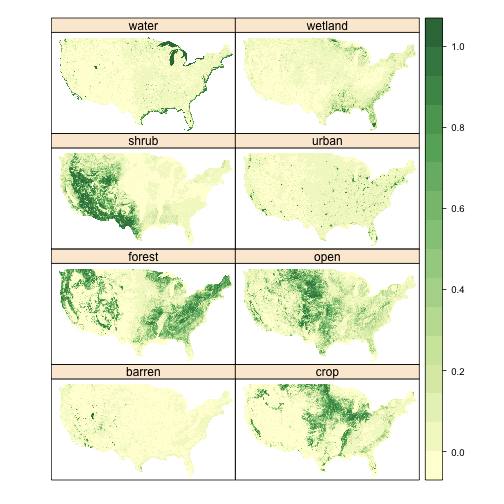
\includegraphics{fig_nlcd}
\end{center} 
\caption{NLCD aggregated cover fractions}
\label{fig:nlcd}
\end{figure} 

\section{Cropland Data Layer (CDL)}
\label{sec:cdl}

\missingfigure{Table or chart showing CDL covereage for various years}

The CDL is only available for a small number of states in 2001.  If
time allows it might be good to compare what is available with our
results as another independent evaluation against a higher-resolution
data set.

\subsection{Reclassification}
\label{sec:cdl-reclass}



%  gdalbuildvrt -tr 0.0002777778 0.0002777778 -te -124.8333 24.5 -66.91667 49.33333 cdl_2001.vrt $(find . -name "*2001*")


\todo{Calculate CDL mask for 5-arcmin cells completely filled}
\todo{Calculate CDL aggregated in GRASS}

\begin{Schunk}
\begin{Sinput}
> cdl <- list( pri= raster( "/gpfs/pads/projects/see/data/raw/cdl/vrt/cdl_2001.vrt"))
> cdlReclassMatrix <- 
+   matrix( c( 83,  83,  0,               # water
+              85,  85,  0,
+              63,  63,  1,               # forest
+                                         # no shrub
+              62,  62,  3,               # open
+              88,  88,  3,
+              87,  87,  4,               # wetland
+               1,  61,  5,               # crop
+              90,  90,  5,
+              82,  82,  6,               # urban
+              84,  84,  6,
+              86,  86,  6),
+                                         # no mosaic
+                                         # no barren
+          ncol= 3, byrow= TRUE)
> cdl  <- mlctReclass( cdl, cdlReclassMatrix, overwrite= overwriteRasters, progress= "text")
> cdl$Amin <- 1
> cdl <- coverFractions( cdl, mosaic= FALSE, overwrite= TRUE, progress="text")
> cdl <- aggregateFractions( cdl, overwrite=TRUE, progress="text")
> cdl_il <- list( pri= raster( "cdl_il_2001.tif"))
> cdl_il <- mlctReclass( cdl_il, cdlReclassMatrix, overwrite= overwriteRasters, progress= "text")
> cdl_il$Amin <- 1
> cdl_il <- coverFractions( cdl_il, mosaic= FALSE, overwrite= TRUE, progress="text")
> cdl_il <- aggregateFractions( cdl_il, overwrite=TRUE, progress="text")
> 
\end{Sinput}
\end{Schunk}



\missingfigure{CDL reclassification table}

\subsection{Aggregation}
\label{sec:cdl-aggr}


\section{Harvested Area and Yields of 175 Crops (175crops2000)}
\label{sec:175crops2000}

\citet{Monfreda2008}

\missingfigure{Table of crops and types reproduced from \citep{Monfreda2008}}

\missingfigure{Summary table of crop aggregations for our model}

\todo{Adress issue of smaller land mask for 175crops2000 and Agland2000}

This data set will provide the information needed to disaggregate the
cropland area taken from Agland2000.  It is not possible to use this
data directly because it reflects only harvested area and so ignores
various types of ancillary agricultural land, rather it will provide
proportions for the disaggregation at the grid cell level.  Rather
than considering the full array of 175 crops we will consider only
corn, soy, wheat, rice, and sugarcane individually, combine other
cereals into their own class, and combine all remaining crops as a
catch-all ``other'' category.  Field crops will be distinguished from
orchard / plantation crops that would likely fall under areas
classified by MLCT as forest or shrub in this step.


%%% Local Variables: 
%%% mode: latex
%%% TeX-master: "thesis"
%%% End: 
